\chapter{Results}\label{chap:Results}

\section{Performance of NLopt}

To test the performance of NLopt, a nonlinear optimization library, trajectories of different length were optimized. Figure \ref{pic:differentGoal} depicts a start vertex and 6 different goal vertices.The figure is in bird's eye perspective and shows a crossing of different hallways. The blue cells represents the floor and the green cells represents the walls. The map was generated with a stereo camera and was not reworked. Therefore some of the cells of the floor which should be occupied/blue are left free. In some of the hallways, there are objects blocking (part of) the way. This passages are tagged with "Bottleneck". Please note that other passages which may look like a bottleneck, such as the top right corner, are not blocked. The green boxes in this passage are part of the ceiling.

\begin{figure}[h]
   \centering
   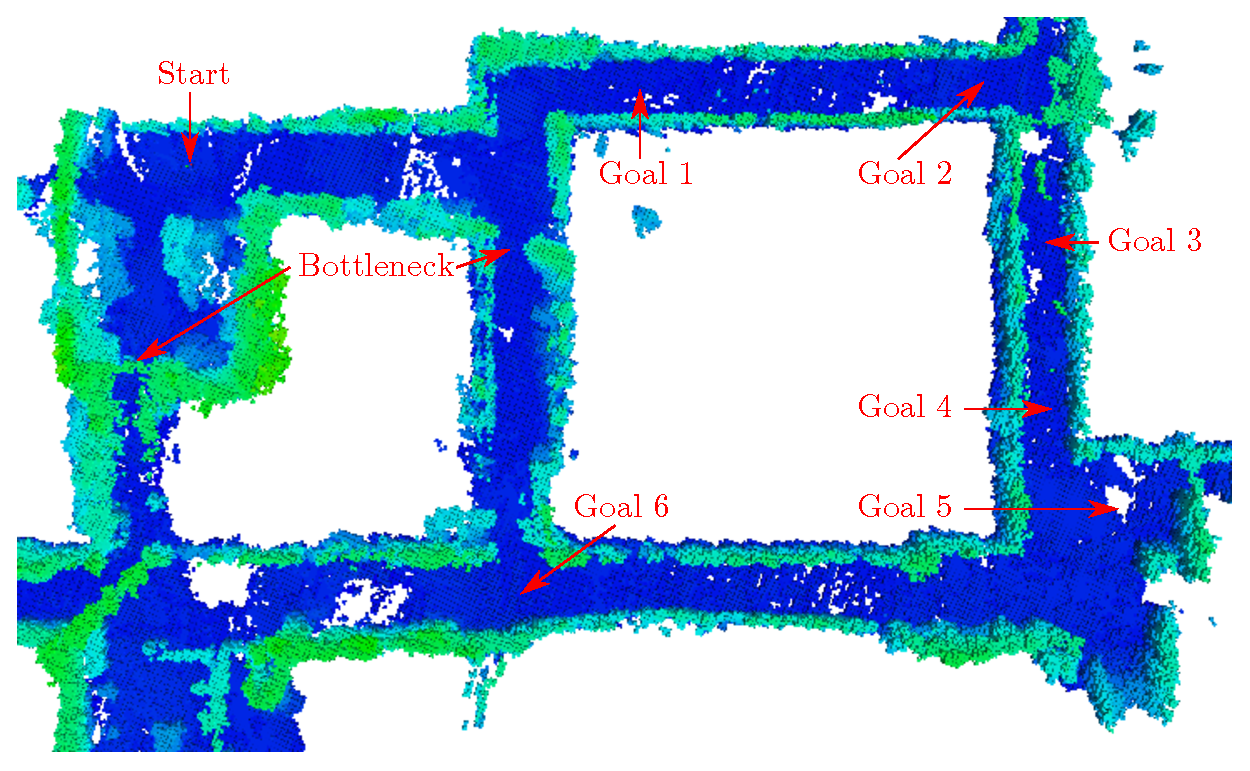
\includegraphics[width=1\textwidth]{pics/ML4.eps}
   \caption{Ein Bild.}
   \label{pic:differentGoal}
\end{figure}

%\begin{figure}[h]
%   \centering
%   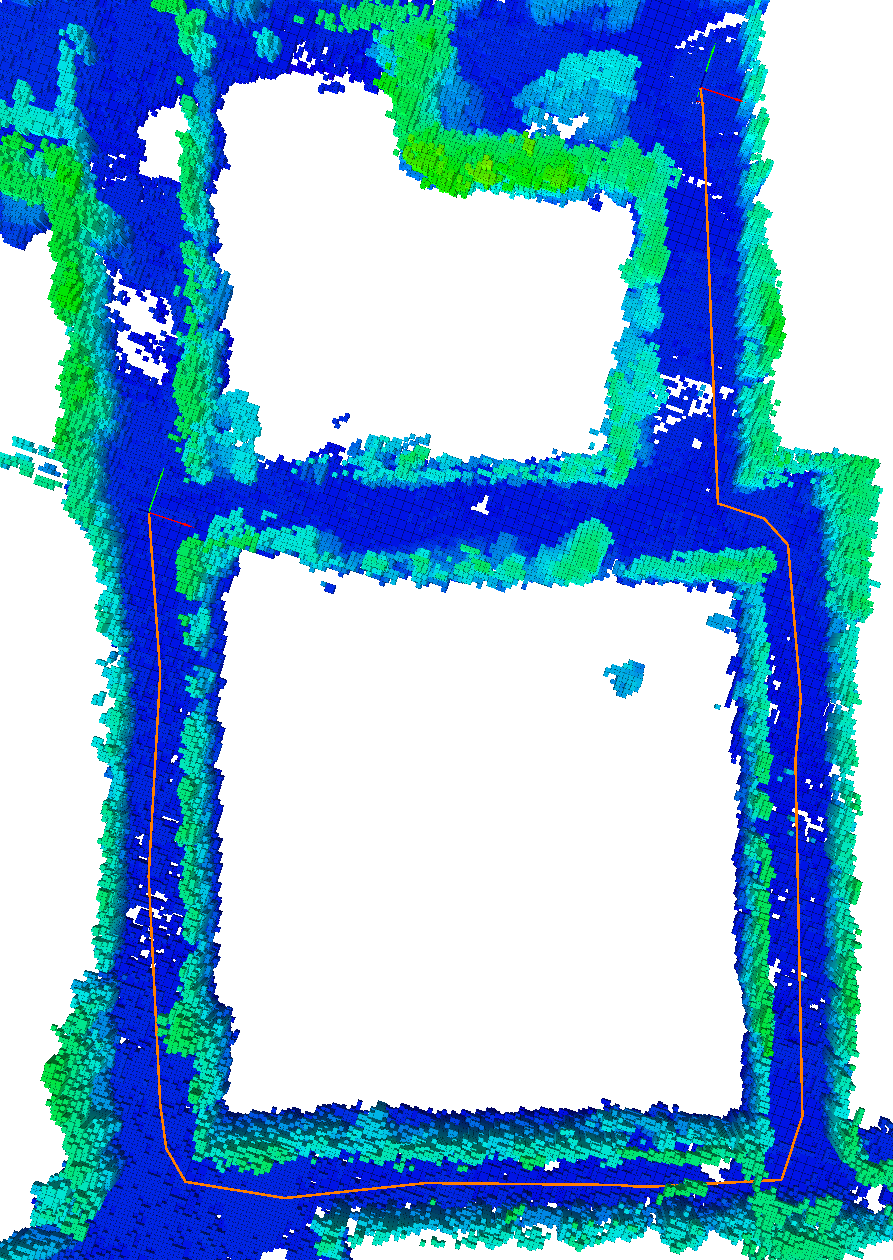
\includegraphics[width=0.5\textwidth]{pics/MapLine.png}
%   \caption{Ein Bild.}
%\end{figure}
%
%
%\begin{figure}[h]
%   \centering
%   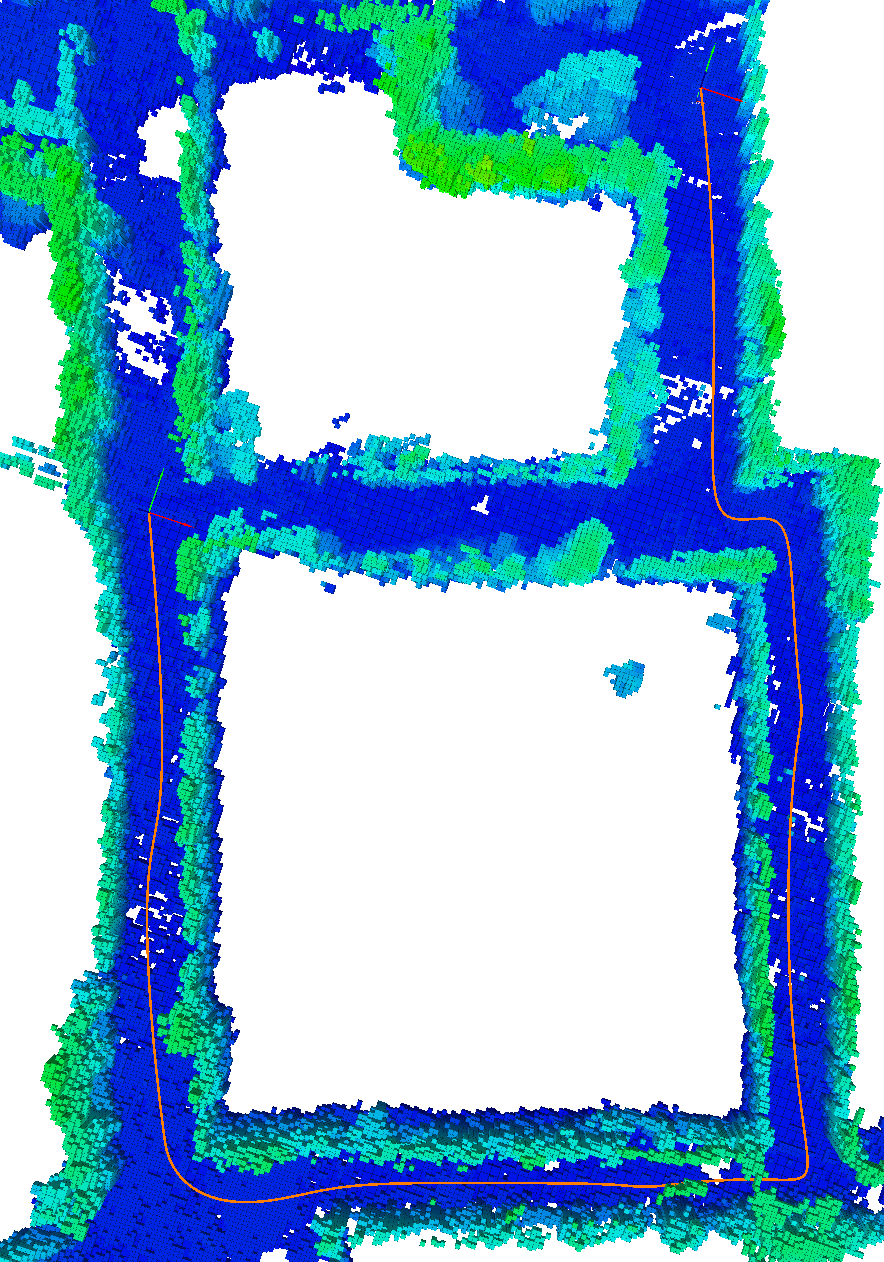
\includegraphics[width=0.5\textwidth]{pics/MapPoly.png}
%   \caption{Ein Bild.}
%\end{figure}

The bottleneck in the center of figure \ref{pic:differentGoal} gets significant for large bounding boxes. If the dimension of the bounding box are larger than $0.5m$ x $0.5m$ x $0.5m$ the trajectory is not able to pass the bottleneck. Hence, a trajectory with a large bounding box has to go all the way around to proceed from the start vertex to "Goal 6" as depicted in figure \ref{pic:Goal6}.


\begin{figure}[ht]
   \centering
   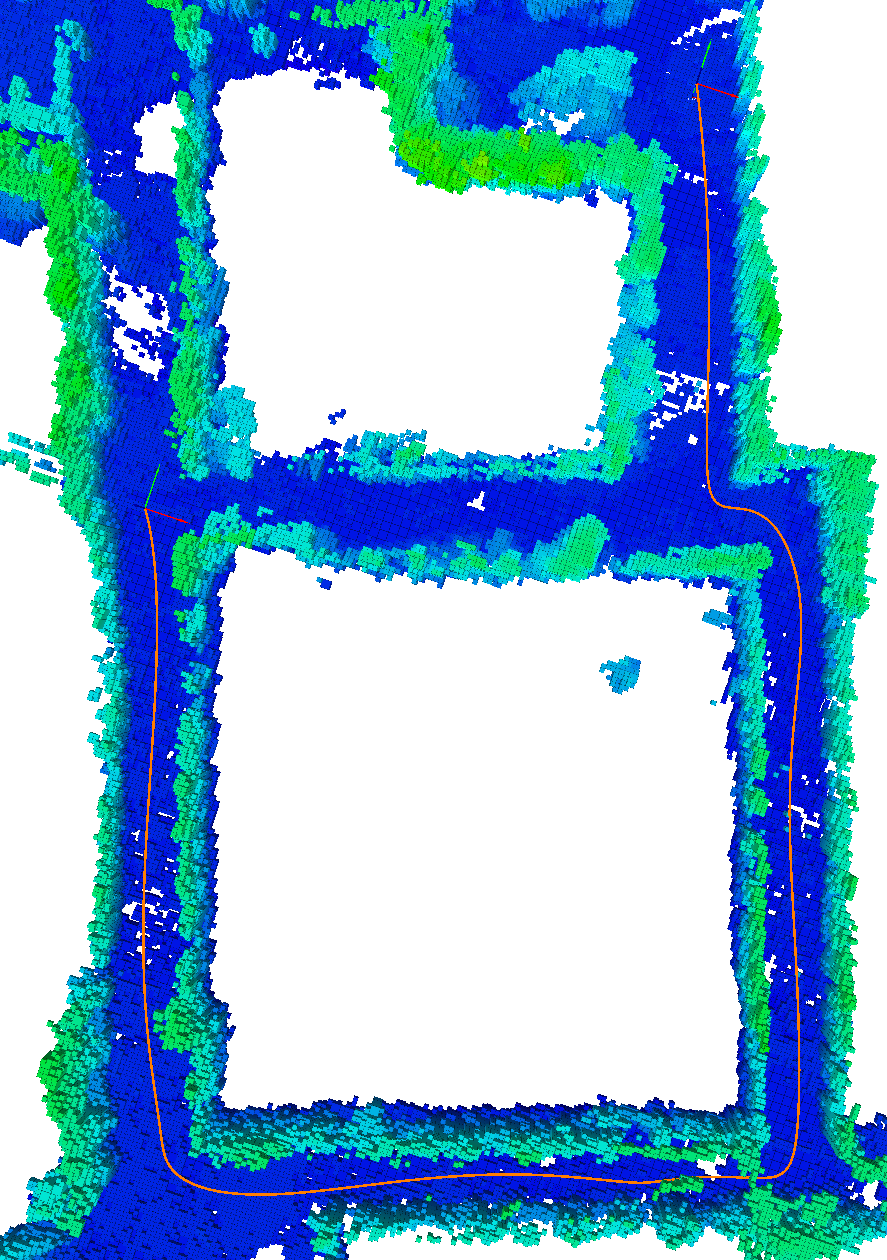
\includegraphics[angle=90, width=1\textwidth]{pics/MapNlopt.png}
   \caption{Ein Bild.}
   \label{pic:Goal6}
\end{figure}

blablabla

\begin{table}[H] 
\begin{center}
    \begin{tabular}{| c | c | c | c | }
    \hline
    Goal Vertex & Number of Segments & Optimization Variables & Optimization Time\\ \hline
   Goal 1 & 1 & 1 & 1\\ \hline
  Goal 2 & 1 & 2& 1\\ \hline
   Goal 3 & 3 & 4& 1\\ \hline
Goal 4 & 3 & 4& 1\\ \hline
Goal 5 & 3 & 4& 1\\ \hline
   Goal 6& 3 & 5& 1\\
    \hline
    \end{tabular}
    \caption{The number of segments of the collision free polynomial solution and the corresponding number of optimization variables. The time needed by NLopt with the ending criteria $f_{rel} = 0.02$}
    \label{tab:MLoptimizationTime}
\end{center}
\end{table}

\section{Reduction of the Optimization Variables}

The results in table \ref{tab:MLoptimizationTime} have shown, that the performance of NLopt decreases with a large amount of optimization variables. In cases where the optimization times is significant (i.e. online planning) the number of optimization parameters can be reduced. The benefits and the drawbacks of a cost function with fewer optimization variables is discussed in the next section.

\newpage

\subsection{Cost Function Without Endpoint Derivatives}

To call to mind, the cost function for the nonlinear optimization is 

\begin{equation}
J_{total} =
\begin{bmatrix}
   d_f \\
  d_p
\end{bmatrix}^T
\begin{bmatrix}
   R_{ff} & R_{fp} \\
  R_{pf} & R_{pp}
\end{bmatrix}
\begin{bmatrix}
   d_f \\
  d_p
\end{bmatrix}
+ k_T \cdot \sum_{i=1}^N T_i
\label{equ:total_cost_Result}
\end{equation}

where the optimization variables are the segment times $T_i$ and the unspecified endpoint derivatives $d_p$. $k_T$ is a user specified weighting factor and $d_f$ is the vector containing the fixed endpoint derivatives. The matrix $R$ resp. the 4 submatrices of $R$ are containing the quadratic snap rearranged according to the fixed and unspecified endpoint derivatives. \newline

As discussed in section \ref{sec:nonlinearopt}, the optimum of this cost function can not be found analytically but with a nonlinear optimization. Only the snap minimized solution of a trajectory with fixed segment times can be computed analytically according to 



\begin{equation}
d_p^* = - R_{pp}^{-1} \cdot R_{fp}^T \cdot d_f
\label{equ:dpstar_Result}
\end{equation}

where the optimal unspecified endpoint derivatives  $d_p^*$ are a function of the fixed derivatives $d_f$ and two of the submatrices ($R_{pp}, R_{fp}$) of $R$. \newline

Since the endpoint derivatives $d_p$ can be found analytically once the segment times $T_i$ are known, $d_p$ can be excluded from the optimization variables. In other words, in every optimization steps the segment times are modified by NLopt. Then $d_p^* $ is computed with the current segment times and the total cost is calculated according to equation \ref{equ:total_cost_Result}. \newline

Recapitulating the new cost function:

\begin{itemize}
  \item The cost function (\ref{equ:total_cost_Result}) remains unchanged .
  \item The segment times $T_i$ are the only optimization variables.
  \item The optimal unspecified endpoint derivatives $d_p^*$ are computed analytically (according to equation \ref{equ:dpstar_Result}) every optimization step with the current segment times.
\end{itemize}

As a consequence of the reduction of the optimization variables, the global minimum of the cost function can not be found in some cases. On the other hand, the nonlinear optimization with $d_p$ and $T_i$ as optimization variables is theoretical able to reach the global minimum of the cost function. Depending on the initial values and on the ending criteria it is possible that the optimization only finds a local minimum. The performance of the two strategies with different optimization variables has therefore to be testes experimentally. \newline

Here comes the comparison!!!!!

\newpage


\section{Performance of the RRT* Algorithm}

In this master thesis, the performance of the RRT* algorithm itself was not improved but the parameters were tuned to serve the nonlinear optimization in an optimal manner.

As mentioned in section \ref{sec:RRTstar}, the calculation time of the RRT* algorithm is mainly defined by the "rewiring" and therefore by the user specified parameter $\gamma$ (used in equation \ref{equ:ballradius}). A good straight line solution, whereas good means a small length of the straight line solution, does not necessarily lead to a good polynomial trajectory. The influence of the user specified parameter $\gamma$ on the final trajectory and the corresponding calculation time is evaluated in this section. \newline
Please call to mind that a small $\gamma$ parameter means little rewiring and a big $\gamma$ parameter means lots of rewiring. The impact of the $\gamma$ parameter can be looked up in figure \ref{pic:smallGamma} and figure \ref{pic:smallBBX}.\newline

Figure \ref{pic:boxplot} depicts the boxplot for different $\gamma$ parameters. Each dataset consists of 15 measurements. On each box, the central mark is the median, the edges of the box are the 25th and 75th percentiles, the whiskers extend to the most extreme
datapoints the algorithm considers to be not outliers, and the outliers are plotted individually. 


\begin{figure}[H]
   \centering
   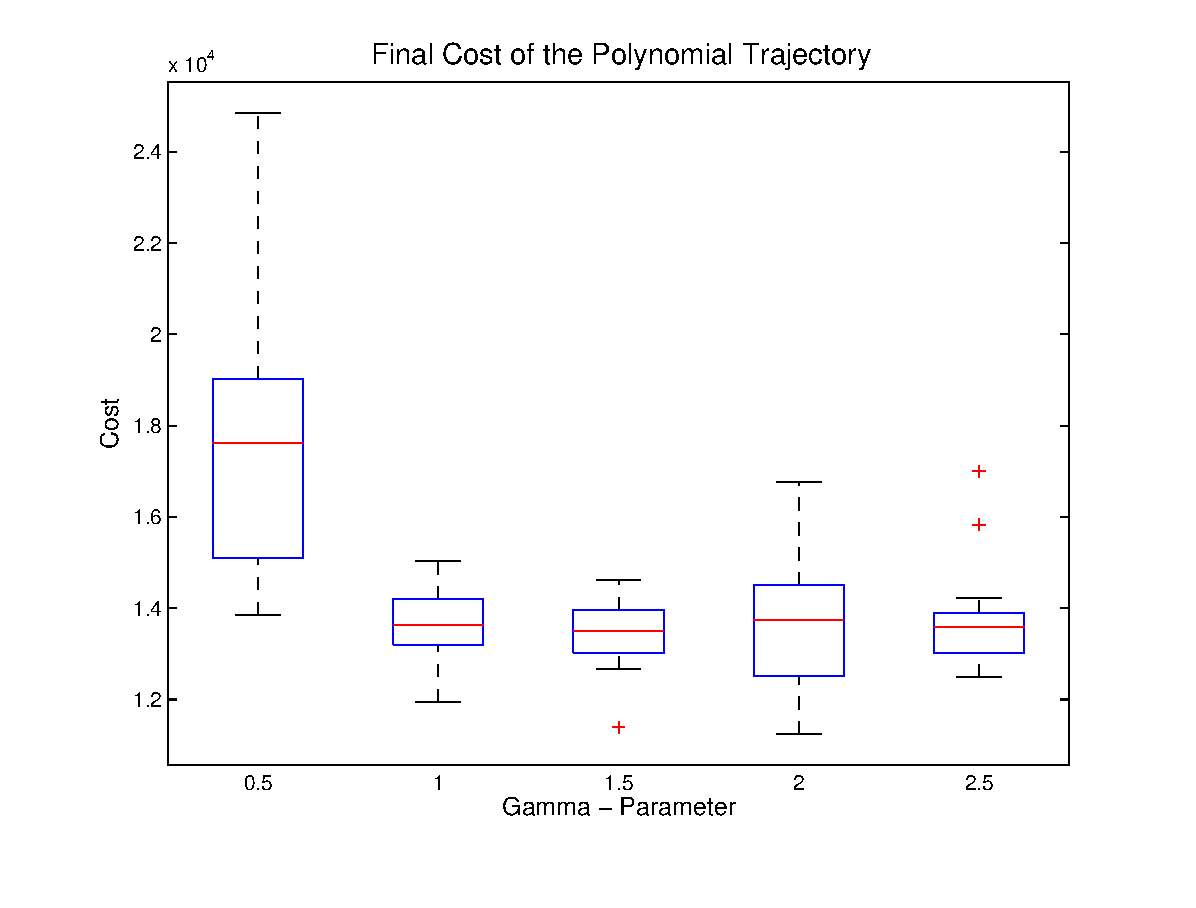
\includegraphics[trim = 14mm 10mm 15mm 0mm,clip,width=1\textwidth]{pics/boxplot1.eps}
   \caption{The $x$-axis depicts different $\gamma$ parameters and the $y$-axis depicts the final cost of the polynomial trajectory. The red mark illustrates the median. }
   \label{pic:boxplot}
\end{figure}


It becomes apparent that the small amount of rewiring associated with $\gamma = 0.5$ is to little to obtain a good polynomial trajectory. The 4 remaining datasets have a similar performance in terms of the final trajectory cost. \newline

The total computational times for the five different $\gamma$ parameters are depicted in figure \ref{pic:boxplot_time}. The total computational time is the combined duration of the RRT* algorithm and the nonlinear optimization.  In contrast to the final cost, the total computational times for $\gamma = 1 $, $\gamma = 1.5$, $\gamma = 2$ and $\gamma = 2.5$ are distinct. 

\begin{figure}[H]
   \centering
   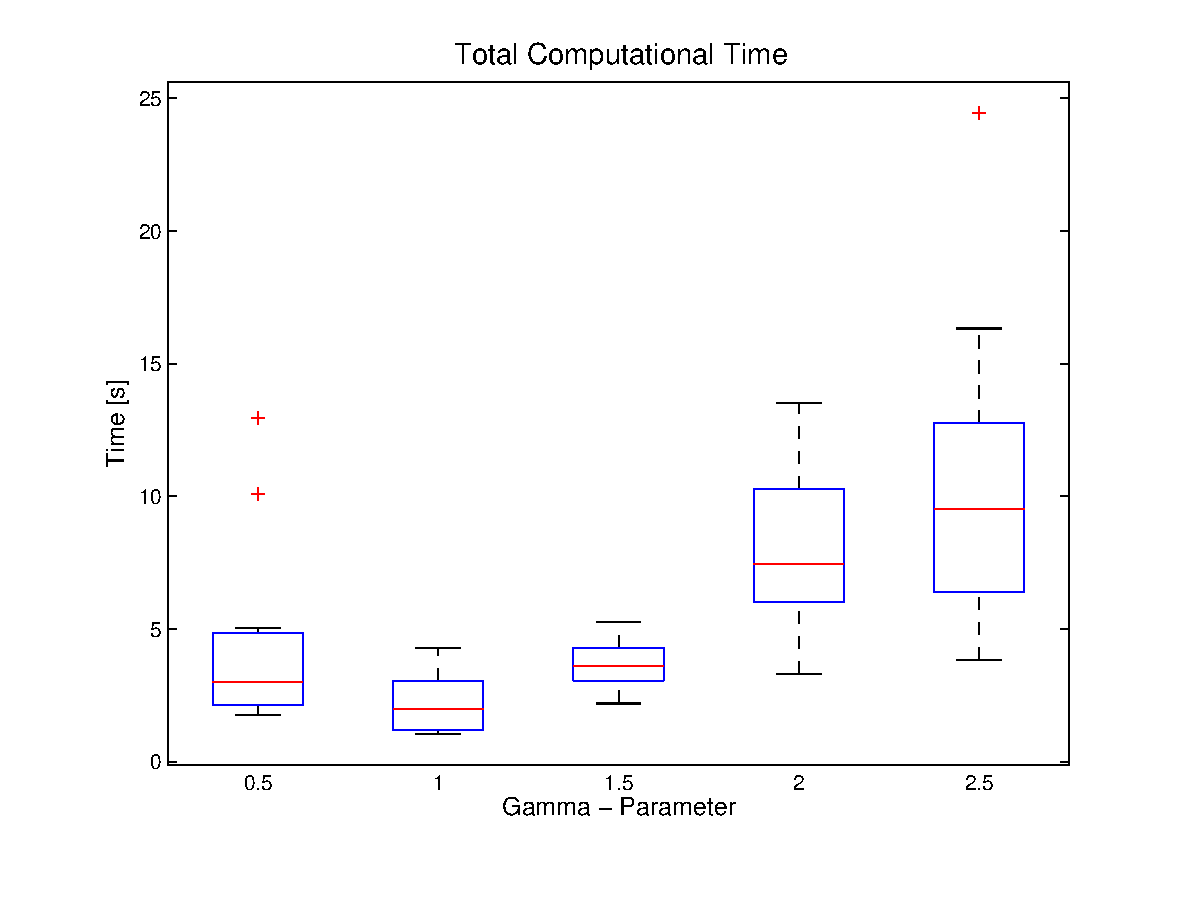
\includegraphics[trim = 14mm 10mm 15mm 0mm,clip,width=1\textwidth]{pics/boxplot_time.eps}
   \caption{The $x$-axis depicts different $\gamma$ parameters and the $y$-axis depicts the total computational time. The red mark illustrates the median.}
   \label{pic:boxplot_time}
\end{figure}

Figure \ref{pic:boxplot_time} shows that the computational time increases significant if $\gamma$ is larger than 1.5. This is simply because the RRT* algorithm needs more time for rewiring. Furthermore, $\gamma = 0.5$ (which is not a good choice sine the final cost is too high) has 2 outliers. In this 2 cases the straight line solution is not enough target-orientated and multible vertex extensions are required to obtain a collision-free trajectory. \newline

Combining the results from figure \ref{pic:boxplot} and figure \ref{pic:boxplot_time}, a $\gamma$ parameter in the range of 1 to 1.5 lead to the best performance.











%
%\begin{figure}
%\centering
%\begin{subfigure}{.5\textwidth}
%  \centering
%  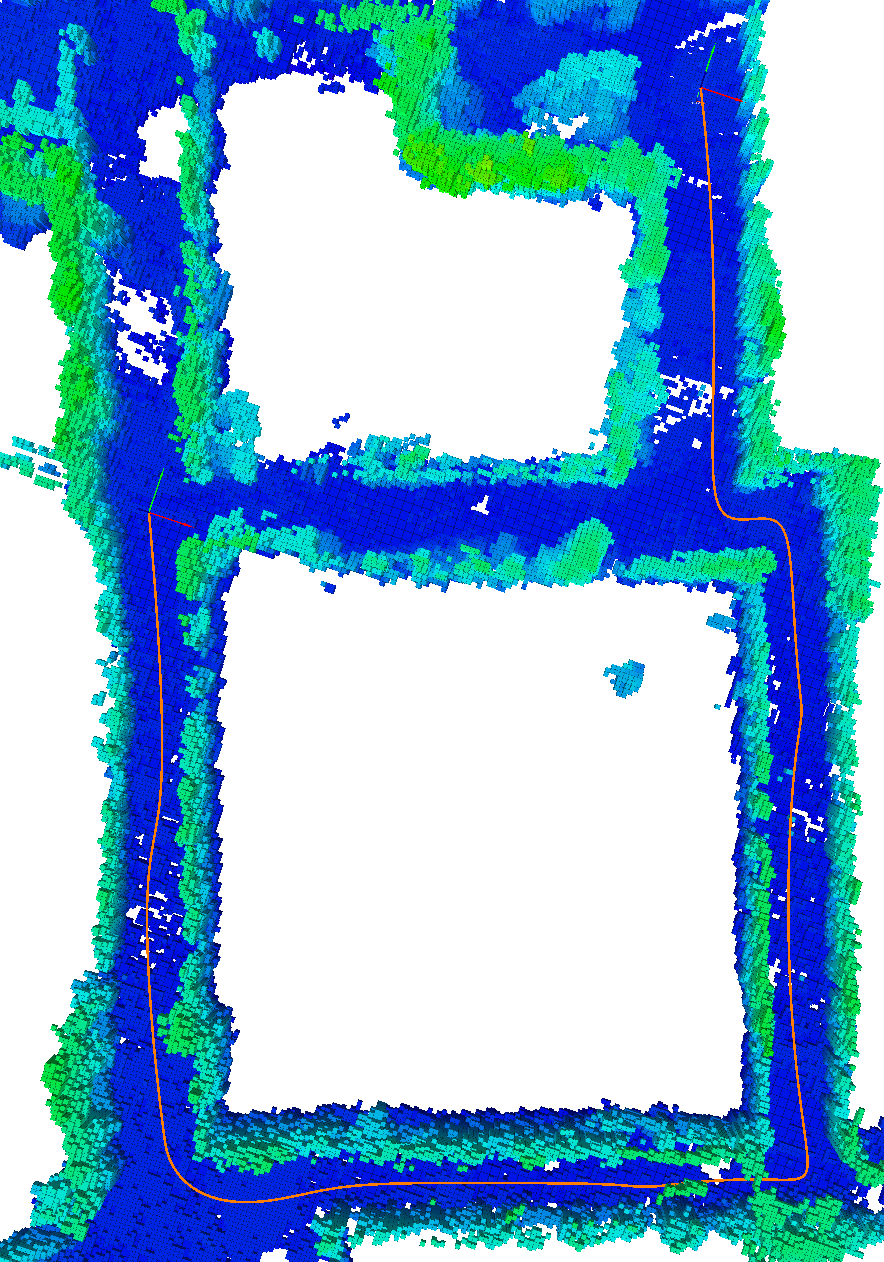
\includegraphics[width=1\linewidth]{pics/MapPoly.png}
%  \caption{A subfigure}
%  \label{fig:sub1}
%\end{subfigure}%
%\begin{subfigure}{.5\textwidth}
%  \centering
%  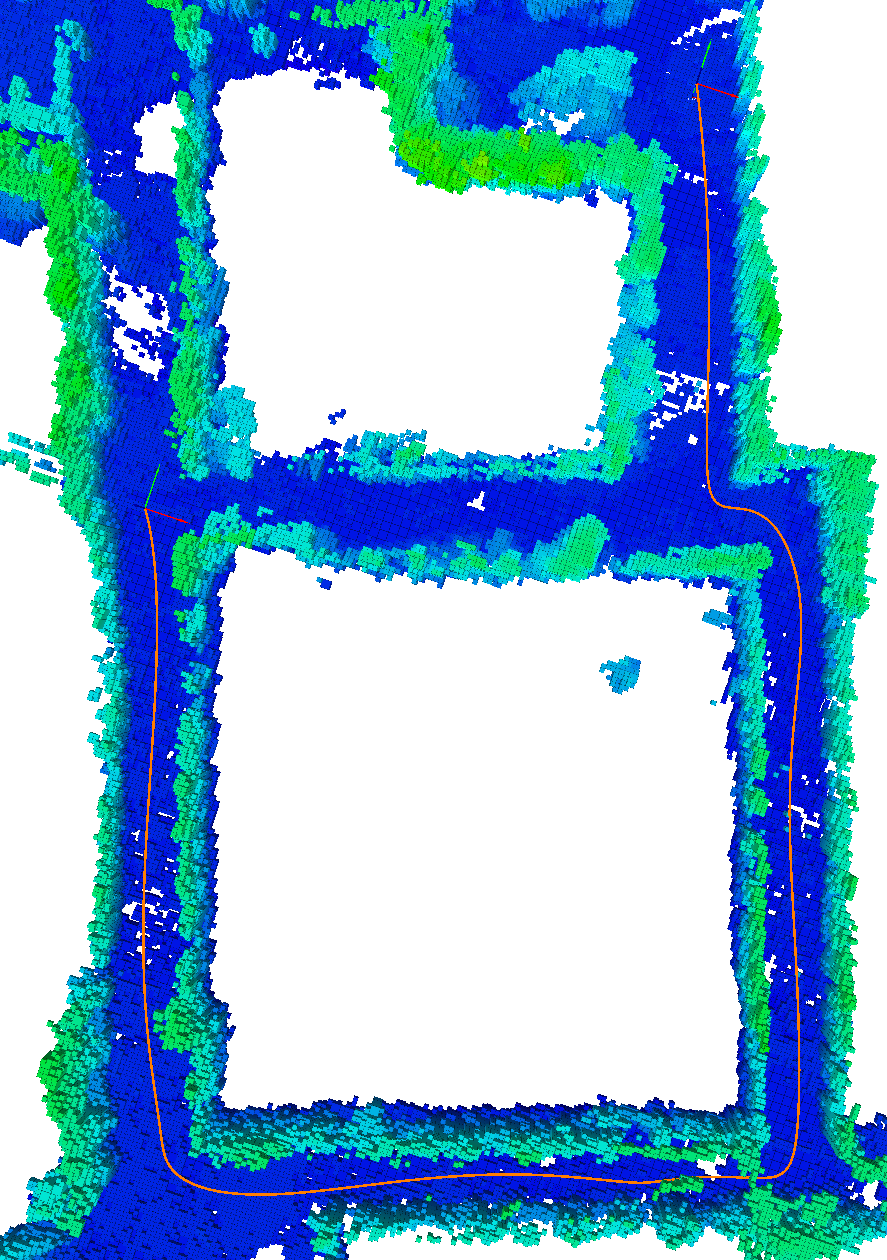
\includegraphics[width=1\linewidth]{pics/MapNlopt.png}
%  \caption{A subfigure}
%  \label{fig:sub2}
%\end{subfigure}
%\caption{A figure with two subfigures}
%\label{fig:test}
%\end{figure}

